\documentclass[12pt,a4paper]{report}
\usepackage[utf8]{inputenc}
\usepackage[french]{babel}
\usepackage[T1]{fontenc}
\usepackage{amsmath}
\usepackage{amsfonts}
\usepackage{amssymb}
\usepackage{graphicx}
\usepackage{appendix}
\usepackage{float} 
\author{Sébastien Hervieu}
\begin{document}

\begin{titlepage}

\newcommand{\HRule}{\rule{\linewidth}{0.5mm}} % Defines a new command for the horizontal lines, change thickness here

\center % Center everything on the page
 
%----------------------------------------------------------------------------------------
%	HEADING SECTIONS
%----------------------------------------------------------------------------------------

\textsc{\LARGE Université de Rennes 1}\\[1cm] 
\textsc{\Large }\\[0.5cm] % Major heading such as course name
\textsc{\large Master 2 Calcul scientifique et modélisation}\\
\textsc{Rapport de Projet de Préstage}\\
%----------------------------------------------------------------------------------------
%	TITLE SECTION
%----------------------------------------------------------------------------------------

\HRule \\[0.4cm]
{ \huge \bfseries Etude et développement d’outils mathématiques pour estimer, en temps réel, le tassage et le volume d’un silo de maïs à partir de capteurs embarqués}\\[0.4cm] 
\HRule \\[1.5cm]
 
%----------------------------------------------------------------------------------------
%	AUTHOR SECTION
%----------------------------------------------------------------------------------------

\begin{minipage}{0.4\textwidth}
\begin{flushleft} \large
\emph{Auteur:}\\
Sébastien \textsc{Hervieu}
\end{flushleft}
\end{minipage}
~
\begin{minipage}{0.4\textwidth}
\begin{flushright} \large
\emph{Professeur:} \\
Fabrice \textsc{Mahé} 
\end{flushright}
\end{minipage}\\[1cm]

% If you don't want a supervisor, uncomment the two lines below and remove the section above
%\Large \emph{Author:}\\
%John \textsc{Smith}\\[3cm] % Your name

%----------------------------------------------------------------------------------------
%	DATE SECTION
%----------------------------------------------------------------------------------------

{\large \today}\\[1cm] % Date, change the \today to a set date if you want to be precise

%----------------------------------------------------------------------------------------
%	LOGO SECTION
%----------------------------------------------------------------------------------------

\includegraphics[height=3cm]{img/logo-tellusenv.png} \\

\includegraphics[height=3cm]{img/univ.jpeg}\\[1cm] % Include a department/university logo - this will require the graphicx package
 
%----------------------------------------------------------------------------------------

\vfill % Fill the rest of the page with whitespace

\end{titlepage}

\tableofcontents
\part{Introduction, Contexte, Objectifs}

\chapter{Introduction}

Le présent chapitre s'attache à présenter le contexte de ce projet de préstage, à savoir l'entreprise dans laquelle le stage se déroulera et le sujet du stage.

Les objectifs du projet de préstage seront enfin présentés.

\section{Présentation de Tellus Environment}
\subsection{Création et Services}
Tellus Environment a été créée en 2012 par Geoffroy ETAIX et Bruno WIRTZ en Juin 2012.

C'est une startup spécialisée dans la cartographie haute  définition des sous-sols et des fond marins, qui propose des services de relevés et mesures nécessaires ainsi que d'analyse de ces données afin d'en permettre l'exploitation par ses clients.

Tellus Environment permet à ses clients de "Cartographier l'invisible pour agir". Elle propose donc de services d'aide à la décision essentiellement à des clients qui interviennent sur le sous-sol et les milieux marins: BTP, aménageurs fonciers, archéologie préventive, agriculture, levée de doute pour la détection précise de réseaux enfouis (eau, gaz, assainissement, télécom) ou de tout autre objet ferreux (épave, vestige de guerre, terre cuite, etc), évaluation avant dépollution de site.

\subsection{Expertises}
La capacité de Tellus Environment à produire des cartographies du sous-sol repose  sur une expertise unique pour le traitement des relevés des sites. Elle a breveté et met en oeuvre le procédé MagSalia, procédé initialement développé par le laboratoire de Mathématiques de L'Université de Bretagne Occidentale.

\paragraph{} Ce procédé appliqué à des relevés magnétiques ...

\paragraph{} Dans sa version sonar multifaisceaux ou lidar, ...

\subsection{Activité Recherche et Développement}
En parallèle de sont activité principalement service, Tellus Environmenent conduit en parallèle une activité Recherche et Développement.

Cette seconde activité peut intevenir soit pour développer de nouvelles techniques de mesure 3D pour améliorer ou étendre sa gamme de service (lidar embarqué sur drone, ...), soit pour apporter son expertise en matière de mise en oeuvre d'acquisition des données et de leur traitement dans la conception d'un produit.

Parmis les projets en cours de cette activité R\&D nous pouvons metntionner les suivants:


\paragraph{Mesure temps réel de tassage de Silo} Il s'agit d'un équipement mettant en oeuvre un Lidar pour mesurer en temps réel le volume d'un silo de maïs afin d'en faire une évaluation fiable du tassage.

\paragraph{Détection en milieu marin zone à risque} Mise en oeuvre de différents capteurs  (Lidar, Sonar, Video IR) pour l'aide à l'accostage de navire en milieux marins risqués.

\paragraph{Détection Automatique GeoRadar} Automatiser l'analyse de signaux radars, en vue d'optimiser le processus de cartographie du sous-sol et l'exploitation des résultats par les différetns acteurs.

\section{Présentation du Stage}
Le sujet du stage, présenté en annexe, interviendra dans le cadre de l'activité R\&D de Tellus Environment, pour améliorer le dispositif existant de mesure en temps réel de mesure de tassage de silo de maïs.

\paragraph{Le tassage de silo de mais} est une activité agricole qui consiste à  tasser de grandes quantités de maïs, généralement dans un silo couloir, en vue d'en permettre la fermentation anaérobie et donc la conservation. Le tassage est une étape primordiale, effectuée à l'aide de tracteurs qui passent de nombreuses fois sur le maïs afin de le compacter. La mesure du tassage est généralement faite au jugé, et est donc relativement imprecise.

\paragraph{Tellus Environnement apporte} une solution qui permet de mesure avec bonne précision, et en temps réel la surface du tas de maïs tassé et d'en déduire le volume. En combinant cette information avec le tonnage de maïs effectivement ensilée, le tassage - c'est dire la densité du maïs tassé - est donc déterminé avec une bien meilleur précision.

\paragraph{Le dispositif existant} est basé sur un capteur laser, le Lidar, qui permet la mesure précise de la surface du tas de maïs. Ce capteur est placé à l'un des angles du silo, et communique ses mesures à un terminal monté dans le cockpit du tracteur.

\begin{figure}[H]
	\centering
	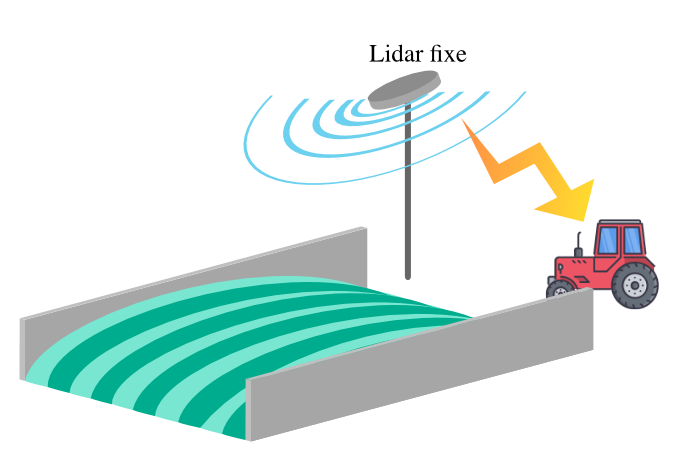
\includegraphics[width=0.7\linewidth]{img/LidarFixe}
	\caption[]{Configuration avec Lidar fixe}
	\label{fig:lidarfixe}
\end{figure}

Le terminal peut donc non seulement indiquer le volume du tas de maïs, mais aussi sa forme et donc indiquer les parties du tas qui auraient besin d'être tassées en priorité.
\newline

Ce système est déjà en exploitation par les clients de Tellus Environment et un retour d'expérience à été effecuté auprès des opérateurs. Le principal défaut remonté de l'équipement lors son exploitation est le temps d'installation du Lidar dans une des coins du silos qui prend en temps certain. Les contraintes en temps des intervenants autour d'un tassage de silo ne sont pas compatibles avec le déploiment d'un instrument sensible comme un Lidar.

\paragraph{La solution à ce problème} envisagée par Tellus Environment est donc de purement et simplement supprimer cette étape d'installation en montant le Lidar directement sur le tracteur de tassage.

\begin{figure}[H]
	\centering
	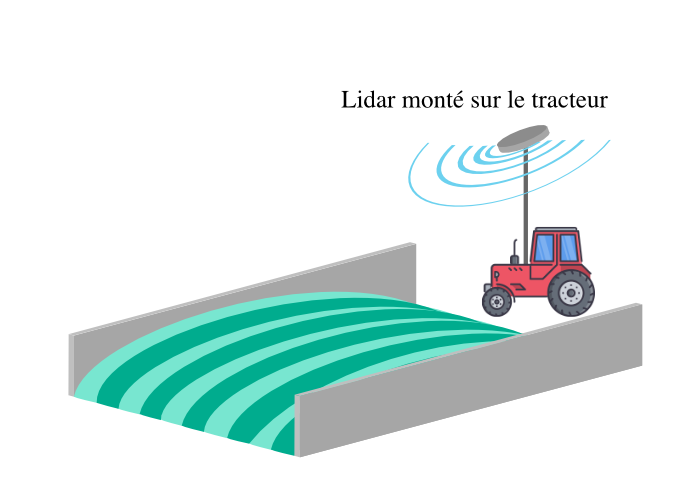
\includegraphics[width=0.7\linewidth]{img/LidarMobile}
	\caption{Configuration avec Lidar monté sur le tracteur}
	\label{fig:lidarmobile}
\end{figure}


\section{Objectifs du projet de pré-stage}
Le projet de pré-stage aura donc les objectifs suivants...

\chapter{Notions d'Agriculture}

L'objectif de ce chapitre est d'introduire l'environnement opérationnel dans lequel le produit final sera déployé, à savoir les chantiers d'ensilage de maïs sur les exploitations d'élevage agricole.

\paragraph{}

L'ensilage a pour but de stocker des fourrages de manière à en permettre la conservation à longue durée et en grande quantité.


\section{Les fourrages: importance économique}

\paragraph{La nourriture: poste financier le plus important pour une exploitation agricole}

\paragraph{Les fourrages: un moyen bon marché pour nourrir les herbivores}

\paragraph{Différents type de fourrages, selon les saisons}
Fourrages verts, ensilages, foin.




\section{Principes de l'ensilage}

\subsection{Fermentation Lactique Anaérobie}

\paragraph{Réaction chimique}

\paragraph{Vertues stérilisatrices, de conservation et nutritionnelles}

\subsection{Les différentes méthodes de conservation des fourrages}

\paragraph{Haylage} Technique qui consiste en l'empilement vertical du fourrage dans des silos-tours verticaux. L'anaérobiose est assurée par l'épaisseur de l'ensemble.
Technique qui requiert des investissements lourds (silo, soufflerie, mécanisme de désillage). Principalement utilisée au Etats-unis.

\paragraph{Enrubannage}

\paragraph{Ensilage par tassement}

\section{Ensilage par tassement: mise en oeuvre}

\subsection{Le chantier d'ensilage}

\paragraph{Vue d'ensemble}

\paragraph{Les différents postes}
\subparagraph{Fourrageuse}
\subparagraph{Navette}
\subparagraph{Tracteur étaleur}
\subparagraph{Tracteur tasseur}

\subsection{Méthodologie du tassage}

\paragraph{Etalement initial de 50cm} par le tracteur étaleur et tassage à 20cm par le tasseur.

\paragraph{Ensuite couche de 20 cm} qui est ensuite tassée à 10cm.

\paragraph{les paramètres cibles}

\subsection{risques d'un tassage mal effectués}

\section{Préparation et la conduite du chantier}

\subsection{Les différents types d'intervenant}
Propriétaires, Groupement agricoles, prestaires de services

\subsection{Gestion de production}
\paragraph{cible de production} prévision de consommation: $x$ kg par jour et par bête $\rightarrow$ quantité d'ensilage à produire.

\paragraph{éviter la surproduction}

\paragraph{permettre la mise en valeur du maïs sur pied restant}




\section{Conclusion}
Nous avons vu que le tassage de silo est une activité stratégique pour une exploitation, qui requiert des moyens lourds, de la planification. C'est de plus une activité très technique, qui est effectuée en parallèle de la récolte, en flux tendu.

\paragraph{}



\chapter{Notions de Détection, Détecteurs}

Notre projet va s'attacher à mesurer un volume d'ensilage à partir d'une plateforme mobile. Cette plateforme doit donc être en mesure de déterminer sa propre position dans le théatre d'opération, de mesurer le silo et de mesure la surface d'ensilage qui y est tassée.

\paragraph{} Ces informations sont recueillies à l'aide de capteurs dont la mise en oeuvre sera une partie majeure du projet.

\section{Notions sur les capteurs}

\subsection{Informations fournies par un capteur de présence}

Mesure de grandeur, fréquence, précision / marge d'erreur.

\paragraph{Portée}
\paragraph{Ouverture} Ouverture en largeur, ouverture en hauteur

\paragraph{Distance, gisement, azimuth}




\section{Les capteurs de position}

\subsection{Odométrie}
L'objet de l'odométrie pour un système mobile est de détecter ses propres déplacements afin de déterminer sa nouvelle position sur la base de capteurs apropriés.


Par exemple, une système mobile à roue peux compter le nombre de tours de roue effectués pour calculer la distance parcourrue.


\subsection{Centrales inertielles}

\subsection{GPS}

\section{Les détecteurs de type "Direction et Portée"}

\subsection{Principes}

\paragraph{Mesures}

\paragraph{Modes d'exploitation}
modes de balayage

\subsection{Les différents types de capteur "Direction et Portée"}

\section{Les capteurs de type "Direction"}
Capteur qui ne sont en mesure de fournir une information que sur la direction de l'objet détecté, sans pouvoir fournir d'information intrinsèque quand à la distance de l'object détecté.

\subsection{Détecteur de présence}

\subsection{Vision par Ordinateur}, analyse d'image, etc



\section{Les détecteurs de type "Portée seulement"}

Détecteurs qui ne fournissent que la portée d'un objet détecté, sans pouvoir fournir d'information précise sur la direction de l'objet en question.



\chapter{Solution Actuelle à Améliorer}

\section{Objectifs initiaux de la version V1}

\section{Présentation de solution}
\subsection{Architecture de la solution}

\subsection{Les sous-systèmes}



\section{Points faibles et axes d'amélioration}

\subsection{Points faibles}

\paragraph{Complexité de mise en oeuvre}
\subparagraph{Installation du Lidar en début de chantier}
\subparagraph{Initialisation de la communication sans fil entre le Lidar et le terminal}

\paragraph{Informations limitées}

\subsection{Axes d'améliorations pour la V2}

\paragraph{Supprimer les facteurs limitants de mise en oeuvre}

\paragraph{Obtenir des informations supplémentaires sur l'état de tassage}

\section{Conclusions}






\part{Outils Importants }

\chapter{Détecteurs en Robotique}

\chapter{Plateforme ROS}

\chapter{Localisation, Cartographie, SLAM}
\section{Positionnement du problème}

\paragraph{Localisation requiert une carte}

\paragraph{Cartographier requiert de connaître sa position}

\paragraph{SLAM permet de résoudre cette problématique "Oeuf et poule"} en mettant à disposition des outils permettant d'exploiter au mieux les informations issues des différents types de capteurs disponibles.

\paragraph{Localisation, vecteur d'état: } système de coordonnées, vecteur d'état.


\section{Maintenir de le vecteur d'état}

\paragraph{Mise en place de la boucle de rafraichissment, filtres de Kalman}

\paragraph{Selectionner des points de repère, les maintenir}

\section{Reconstituer l'environnement}


\chapter{Mesurer le tassage}

\section{Modéliser une surface en 3D}

\section{Calculer le volume à partir d'une surface 3D mesurée}


\chapter{Prototypage}
\section{Prototypage Scientifique des Algorithmes}
\subsection{Matlab}
\subsection{Python}
\section{Prototype de mise en œuvre}
\subsection{Plateforme ROS}
\subsection{Mise en oeuvre en C et/ou C++}

\part{Application Numérique}

\chapter{Application Numérique}
L'objectif de cette partie est de concevoir et mettre en oeuvre un algorithme de détection de forme à partir d'un nuage de points, pouvant être issu d'un capteur de type "portée et direction".

\begin{enumerate}
\item
Produire des données de référence à partir de modèle de structure 3D connus.
\item
Introduire bruit gaussien sur les points, de manière à produire un nuage de points bruité
\item
Développer un technique d'inversion permettant de détecter la forme
et les dimensions des structures à partir des nuages de points
bruités
\item
Evaluer les marges d'erreur des modèles inversés
\item
Dégager les axes de progression en terme de performance de calcul:
l'objectif est d'obtenir des outils qui produisent des résultats en
quelques secondes.
\end{enumerate}

\part{Conclusions du Projet Préliminaire au Stage}
  
\chapter{Objectifs SMART du Stage}
\chapter{Conclusion}

\begin{appendix}
\chapter{Sujet de stage}
\end{appendix}



\end{document}
